\documentclass[conference]{IEEEtran}

\usepackage{amsmath,amssymb,amsfonts}
\usepackage{algorithmic}
\usepackage{algorithm}
\usepackage{graphicx}
\usepackage{textcomp}
\usepackage{xcolor}
\usepackage{booktabs}
\usepackage{cite}
\usepackage{multirow}
\usepackage{bm}
\usepackage{enumitem}

\newcommand{\vect}[1]{\bm{#1}}
\newcommand{\posv}[1]{\vect{p}_{#1}}
\newcommand{\bore}[1]{\hat{\vect{b}}_{#1}}
\newcommand{\dB}{\,\mathrm{dB}}
\newcommand{\dBi}{\,\mathrm{dBi}}
\newcommand{\dBm}{\,\mathrm{dBm}}

\begin{document}

% \title{Analytic Geometry-Based Heuristic for User-Aware UAV Deployment with Interference Management}

\title{Geometry-Based UAV Communication Deployment for Coverage and Interference Management}

% \author{
% \IEEEauthorblockN{Abdulrahman Almanea}
% \IEEEauthorblockA{King Abdullah University of Science and Technology (KAUST)\\
% Thuwal, Saudi Arabia}

% \IEEEauthorblockN{Balsam Alkouz}
% \IEEEauthorblockA{King Abdullah University of Science and Technology (KAUST)\\
% Thuwal, Saudi Arabia}

% \IEEEauthorblockN{Basem Shihada}
% \IEEEauthorblockA{King Abdullah University of Science and Technology (KAUST)\\
% Thuwal, Saudi Arabia}
% }

\author{
\IEEEauthorblockN{Abdulrahman Almanea, Balsam Alkouz, and Basem Shihada}
\IEEEauthorblockA{King Abdullah University of Science and Technology (KAUST)\\
Thuwal, Saudi Arabia\\
\{abdulrahman.almanea, balsam.alkouz, basem.shihada\}@kaust.edu.sa}
}


\maketitle

\begin{abstract}
Unmanned aerial vehicle (UAV) base stations are a promising solution for restoring connectivity in disaster scenarios where terrestrial infrastructure is destroyed, overloaded, or absent. However, a single UAV has limited capacity, and large numbers of ground users may simultaneously require connectivity, necessitating multiple drones operating as a swarm. Deploying such a swarm requires jointly determining how many drones to deploy and where to place them, balancing coverage against inter-drone interference. Existing approaches either rely on computationally expensive metaheuristic optimizers or ignore the directional, geometry-dependent interference created by antenna radiation patterns. We propose an analytic geometry-based heuristic that exploits closed-form relationships between user cluster geometry, antenna beamwidth, and inter-drone topology to derive complete deployments. The \emph{analytic heuristic} uses K-means clustering for horizontal placement, a beam-footprint formula for per-drone altitude, nadir-pointing for the userlink antenna, and a minimum spanning tree for backhaul pointing. Evaluation over 144 synthetic configurations and 24 real-world Telecom Italia snapshots shows that the analytic heuristic achieves a $+25$ percentage point mean coverage gain over a K-means baseline at negligible computational cost, with robustness to real-world spatial heterogeneity.

\end{abstract}

\begin{IEEEkeywords}
UAV Communications, UAV Assisted Networks, Antenna Radiation Pattern, Inter-drone Interference, Geometry-based Deployment
\end{IEEEkeywords}

%----------------------------------------------------------------------
\section{Introduction}
\label{sec:intro}
%----------------------------------------------------------------------

Unmanned aerial vehicle (UAV) base stations are a promising solution for providing connectivity in scenarios where terrestrial infrastructure is unavailable, overloaded, or impractical, such as disaster relief, temporary mass events, or coverage extension in remote and underserved areas~\cite{qiu2019,elhammouti2019,hydher2020}.
When multiple drones operate in close proximity sharing spectrum resources, inter-drone interference becomes a dominant performance-limiting factor~\cite{betchersbrolla2025}. The deployment problem, deciding \emph{how many} drones to deploy, \emph{where} to place them, and \emph{how} to orient their antennas, is a tradeoff: more drones increase spatial coverage but also increase mutual interference.

Existing approaches include heuristic placement methods such as K-means clustering~\cite{consul2024}, distributed methods for joint multi-UAV 3D placement and user association~\cite{elhammouti2019}, CNN-based rapid deployment methods for multi-UAV networks~\cite{wang2024}, and optimization-driven methods for multi-UAV deployment with jointly considered user access and backhaul connectivity~\cite{wang2025multiuav}. However, these methods typically do not exploit directional antenna geometry to derive closed-form altitude and orientation rules.
% Existing approaches include heuristic placement methods such as K-means clustering~\cite{consul2024}, optimization-driven methods for multi-UAV deployment with jointly considered user access and backhaul connectivity~\cite{wang2025multiuav}, and electromagnetic-compatibility-aware UAV formation adjustment methods~\cite{huang2025}. However, these methods typically do not exploit directional antenna geometry to derive closed-form altitude and orientation rules.

This paper bridges the gap by proposing an \emph{analytic geometry-based heuristic} that (1) derives a complete deployment (positions, altitudes, and antenna orientations) from closed-form geometric relationships in milliseconds, (2) explicitly accounts for directional antenna patterns and inter-drone interference through beam-footprint matching and minimum spanning tree (MST) backhaul topology, and (3) requires no iterative optimization or objective function evaluations.

The key observation motivating our approach is that ground users rarely distribute uniformly; they naturally form spatial clusters around shelters, gathering points, or areas of interest. When a drone is placed above a cluster, the spatial extent of that cluster directly determines how high the drone should fly: a dense cluster requires a lower altitude to focus the beam, while a spread-out cluster requires a higher altitude for broader coverage. Furthermore, since each drone is placed directly above its cluster centroid, nadir-pointing naturally maximises the fraction of cluster users inside the main lobe, with no tilt required. Finally, the 3D positions of deployed drones define a natural graph structure, and a minimum spanning tree over this graph provides an efficient backhaul topology that aligns antenna pointing with actual communication paths []. Together, these observations reduce the deployment problem to a set of closed-form geometric computations, eliminating the need for iterative optimization entirely. Fig.~\ref{fig:system} illustrates the proposed deployment setting. 

The main contributions of this paper are summarized as follows:
\begin{itemize}
    \item We present a geometry-dependent interference model that jointly accounts for directional antenna patterns and probabilistic air-to-ground channels in a multi-UAV deployment setting.
    \item We propose an analytic geometry-based heuristic that derives complete UAV swarm deployments from closed-form geometric relationships with no iterative optimization.
    % \item We validate the nadir-pointing UL orientation through a per-drone tilt--azimuth sweep ($1^\circ$/$5^\circ$ resolution, 36 configurations), confirming that nadir-pointing leaves on average only $0.4$ percentage points of coverage to per-drone optimisation.
    \item We evaluate 144 synthetic configurations (three user distributions) and 5 real-world Telecom Italia snapshots at high user density.
\end{itemize}



%----------------------------------------------------------------------
\section{System Model}
\label{sec:system}
%----------------------------------------------------------------------

We consider a square area of side $L = 2000$\,m in which $M$ ground users require connectivity from a fleet of $N$ UAV base stations. Each UAV~$j$ is characterized by its 3D position $\posv{j} = (x_j, y_j, z_j)$ and the orientations of two antennas: a userlink (UL) antenna serving ground users with tilt $\tau_j^{\mathrm{UL}}$ and azimuth $\alpha_j^{\mathrm{UL}}$, and a backhaul (BH) antenna for inter-drone communication with tilt $\tau_j^{\mathrm{bh}}$ and azimuth $\alpha_j^{\mathrm{bh}}$.

\begin{figure}[t]
\centering
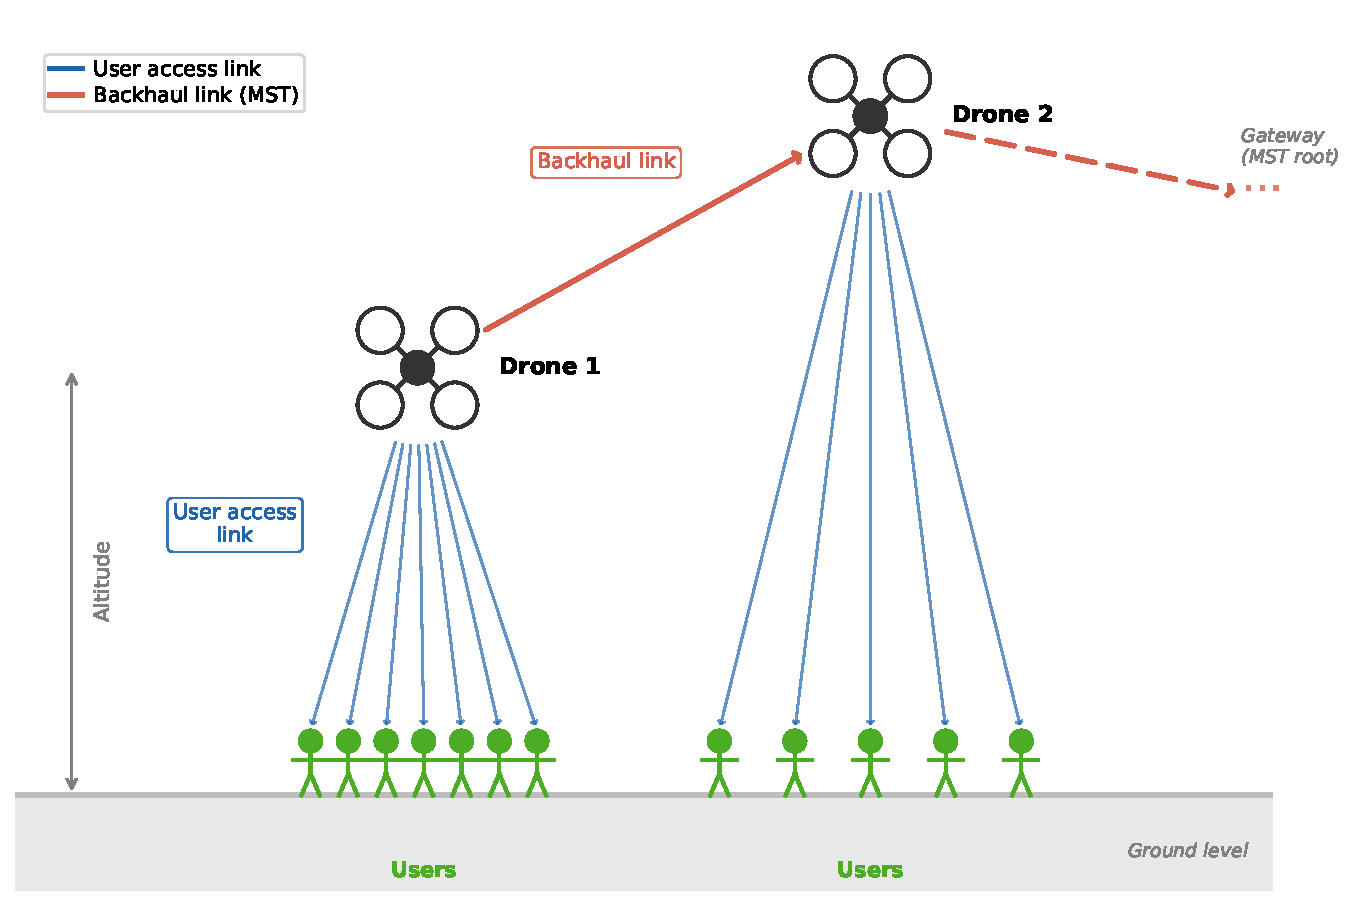
\includegraphics[width=\columnwidth]{figures/environment_figure.pdf}
\caption{Illustration of the deployment setting. Each drone serves a cluster of ground users through a downlink access antenna, while backhaul connectivity is maintained through an inter-drone minimum spanning tree rooted at the gateway. Drone altitude is adapted to the user cluster geometry.}
\label{fig:system}
\end{figure}

\subsection{User-Aware Deployment}

We assume that user positions are known prior to deployment. This models scenarios where user locations are obtained from cellular network historical records, crowd-sensing, or aerial imagery before the drone fleet is launched. Each deployment method receives the user layout as input and produces a complete configuration. %The same user layout is used for both deployment planning and performance evaluation.

\subsection{Antenna Radiation Model}

We adopt a parametric single-element pattern inspired by 3GPP~TR~38.901~\cite{3gpp38901}:
\begin{equation}
\label{eq:antenna_gain}
G(\theta) = G_{\max} - \min\!\left(12\left(\frac{\theta}{\theta_{3\mathrm{dB}}}\right)^{\!2},\; A_{\mathrm{SLA}}\right) \quad [\dBi]
\end{equation}
where $\theta$ is the off-boresight angle, $G_{\max}$ is the peak gain, $\theta_{3\mathrm{dB}}$ is the full $-3\dB$ beamwidth, and $A_{\mathrm{SLA}}$ is the sidelobe attenuation.
The pattern is azimuthally symmetric around the boresight axis.

The off-boresight angle from drone~$j$ toward target position~$\vect{q}$ is:
\begin{equation}
\theta_{j} = \arccos\!\left(\bore{j} \cdot \hat{\vect{d}}_{j}\right)
\end{equation}
where $\bore{j}$ is the boresight unit vector determined by the tilt and azimuth:
\begin{equation}
\bore{j} = \begin{pmatrix} \sin\tau_j\cos\alpha_j \\ \sin\tau_j\sin\alpha_j \\ -\cos\tau_j \end{pmatrix}
\end{equation}
with $\tau_j = 0$ corresponding to nadir.
We use a UL antenna with $(G_{\max} = 18\dBi,\; \theta_{3\mathrm{dB}} = 60^\circ,\; A_{\mathrm{SLA}} = 20\dB)$ and a BH antenna with $(G_{\max} = 12\dBi,\; \theta_{3\mathrm{dB}} = 30^\circ,\; A_{\mathrm{SLA}} = 25\dB)$.

\subsection{Channel Model}

For air-to-ground links, we use the probabilistic LoS model of Al-Hourani et~al.~\cite{alhourani2014}:
\begin{equation}
P_{\mathrm{LoS}}(\phi) = \frac{1}{1 + a\,\exp\!\big(-b\,(\phi_{\mathrm{deg}} - a)\big)}
\end{equation}
with urban parameters $a = 9.61$, $b = 0.16$.
The average path loss combines free-space path loss with probabilistically weighted excess losses:
\begin{equation}
\mathrm{PL}(d, \phi) = 20\log_{10}\!\left(\frac{4\pi d f_c}{c}\right) + P_{\mathrm{LoS}}\,\eta_{\mathrm{LoS}} + (1 - P_{\mathrm{LoS}})\,\eta_{\mathrm{NLoS}}
\end{equation}
with $\eta_{\mathrm{LoS}} = 1\dB$, $\eta_{\mathrm{NLoS}} = 20\dB$, and $f_c = 2$\,GHz.
Air-to-air backhaul links use pure free-space path loss.

\subsection{SINR and Interference}

Each user~$u$ is associated with the nearest drone $j^*(u)$.
The userlink SINR is:
\begin{equation}
\mathrm{SINR}_u = \frac{P_{j^*,u}^{\mathrm{rx}}}{\sigma^2 + \sum_{j \neq j^*} P_{j,u}^{\mathrm{rx}}}
\end{equation}
where $P_{j,u}^{\mathrm{rx}} = P_{\mathrm{tx}}^{\mathrm{UL}} \cdot G^{\mathrm{UL}}(\theta_{ju}) \cdot 10^{-\mathrm{PL}/10}$ and $\sigma^2$ is the thermal noise power ($N_0 = -174\dBm$/Hz, $B = 10$\,MHz).
All drones share a single userlink frequency band (worst-case interference).

The total inter-drone backhaul interference accounts for directional gain at both ends:
\begin{equation}
I_{\mathrm{total}}^{\mathrm{bh}} = \sum_{j=1}^{N}\sum_{\substack{i=1\\i>j}}^{N} P_{\mathrm{tx}}^{\mathrm{bh}} \cdot G^{\mathrm{bh}}(\theta_{ji}^{\mathrm{tx}}) \cdot G^{\mathrm{bh}}(\theta_{ij}^{\mathrm{rx}}) \cdot L_{\mathrm{a2a}}(d_{ji})
\end{equation}
This geometry-dependent interference is the key quantity that deployment methods must manage.

\subsection{Performance Metrics}

A user is \emph{covered} if $\mathrm{SINR}_u \geq \gamma_r = 3\dB$, a lenient minimum-connectivity requirement below the range swept by Khuwaja et al.~\cite{khuwaja2019}, whose analysis shows that coverage area is sensitive to the choice of $\gamma_r$.
We focus on coverage rather than throughput, since in emergency deployments the primary objective is to establish minimum connectivity for as many users as possible.
The primary metric is coverage percentage, defined as the fraction of covered users.
%----------------------------------------------------------------------
\section{Deployment Methods}
\label{sec:methods}
%----------------------------------------------------------------------

We compare two deployment methods, both user-aware, that share the same horizontal placement (K-means centroids) but differ in how they set drone altitudes and antenna orientations.
The K-means baseline uses a fixed altitude with nadir-pointing antennas, while the analytic heuristic derives altitude and orientations from the antenna geometry.

%\begin{table}[h]
%\centering
%\caption{Deployment Method Comparison}
%\label{tab:methods}
%\begin{tabular}{@{}lcccc@{}}
%\toprule
%Method & Positions & Altitude & UL Orient & BH Orient \\
%\midrule
%K-means & centroids & fixed 150\,m & nadir & MST \\
%Analytic & centroids & beam-match & nadir & MST \\
%%Greedy & grid search & beam-match & centroid & MST \\
%\bottomrule
%\end{tabular}
%\end{table}

\subsection{K-means Baseline}

The baseline places drones at the K-means cluster centroids of the known user positions.
All drones fly at a fixed altitude of 150\,m with nadir-pointing UL antennas ($\tau^{\mathrm{UL}} = 0$).
BH antennas are oriented via MST (Section~\ref{sec:analytic}, Step~4).
This method represents a standard user-aware placement with no geometric awareness of the antenna patterns.

\subsection{Analytic Geometry-Based Heuristic}
\label{sec:analytic}

The proposed analytic heuristic derives a complete deployment through four closed-form steps, summarized in Algorithm~\ref{alg:analytic}.

\subsubsection{Step 1: Horizontal Placement via K-means}
Since each drone serves a subset of users, the natural position that minimises the average distance to its assigned users is their centroid, making K-means, which partitions users into $K{=}N$ clusters and returns exactly those centroids, the natural choice for horizontal placement [Line~1].
Drone $(x, y)$ positions are set at the K-means centroids of the user positions, identical to the baseline.
This places each drone above the center of mass of its assigned user cluster.

\subsubsection{Step 2: Altitude from Beam-Footprint Matching}
\label{sec:altitude}

Altitude has a strong effect on aerial-link performance and interference, making height selection a key design variable in UAV-assisted networks \cite{zhou2019}. In our heuristic, each drone's altitude is chosen so that the UL antenna's $-3$\,dB footprint matches the spatial extent of its assigned user cluster.

For a nadir-pointing antenna with half-beamwidth $\theta_{3\mathrm{dB}}/2$, the ground-footprint radius is $z \tan(\theta_{3\mathrm{dB}}/2).$
We set this radius equal to the cluster spread $\sigma_j$ (the empirical standard deviation of user positions in cluster $j$). This gives the altitude rule
\begin{equation}
\label{eq:altitude}
z_j = \frac{\sigma_j}{\tan(\theta_{3\mathrm{dB}}/2)},
\end{equation}
which is then clamped to the feasible range $[50, 300]$\,m.

This rule adapts altitude to the geometry of the assigned users. Dense clusters, with small $\sigma_j$, are served from lower altitudes, producing tighter footprints and stronger received signal strength. More spatially dispersed clusters require higher altitudes so that the illuminated area remains wide enough to cover the users assigned to that drone.
%A drone that flies too high wastes signal power on empty ground, while one that flies too low illuminates only a fraction of its cluster; the right altitude is therefore the one that makes the antenna's $-3\,$dB footprint exactly cover the cluster [Lines~3--4].
%Each drone's altitude $(z)$ is set so that the UL antenna's $-3\dB$ beam footprint matches the spatial extent of its user cluster.
%For a nadir-pointing antenna with half-beamwidth $\theta_{3\mathrm{dB}}/2$, the ground footprint radius is $z \tan(\theta_{3\mathrm{dB}}/2)$.
%Setting this equal to the cluster spread $\sigma_j$ (empirical standard deviation of user positions within cluster $j$):
%\begin{equation}
%\label{eq:altitude}
%z_j = \frac{\sigma_j}{\tan(\theta_{3\mathrm{dB}}/2)}
%\end{equation}
% clamped to $[50, 300]$\,m.
% Dense clusters (small $\sigma_j$) get lower altitudes, yielding tighter beams and stronger per-user signal; spread-out clusters get higher altitudes to maintain broad coverage.

\subsubsection{Step 3: Userlink Orientation}
Because K-means places each drone at the centroid of its assigned user cluster, the drone's horizontal position $(x_j, y_j)$ coincides exactly with the ground centroid $(\bar{x}_j, \bar{y}_j)$ of that cluster [Line~5].
Consequently, pointing the UL boresight toward the ground centroid always reduces to nadir:
\begin{equation}
\tau_j^{\mathrm{UL}} = 0 \quad (\text{nadir})
\end{equation}
No tilt computation is needed; the UL antenna is simply set to nadir.
This means the only difference between the K-means baseline and the analytic heuristic is the altitude assignment (Step~2): both methods use nadir-pointing UL antennas and MST backhaul, but the analytic heuristic adapts each drone's altitude to its cluster geometry rather than fixing it at 150\,m.

\subsubsection{Step 4: Backhaul Orientation via MST}
Inter-drone interference grows rapidly when backhaul beams are pointed arbitrarily; a spanning-tree topology guarantees connectivity with the minimum number of active links, and rooting it at the drone nearest the ground infrastructure keeps the uplink path short [Lines~7--11].
A minimum spanning tree (MST) is computed over the 3D drone positions using Euclidean distance. The tree is rooted at the \emph{gateway drone}, defined as the drone whose horizontal position $(x_j, y_j)$ is closest to the area origin $(0,0)$, placing it at the edge of the deployment area nearest to the ground infrastructure.
Each non-gateway drone points its BH antenna toward its MST parent. The gateway drone points its BH antenna horizontally ($\tau_g^{\mathrm{bh}} = \pi/2$, $\alpha_g^{\mathrm{bh}} = 0$) toward the ground base station. This produces a connected tree topology that minimises total backhaul link distance and aligns BH antennas along actual communication paths.

\begin{algorithm}[ht]
\caption{Analytic Geometry-Based Deployment}
\label{alg:analytic}
\begin{algorithmic}[1]
\REQUIRE User positions $\{(x_u, y_u, 0)\}_{u=1}^{M}$, fleet size $N$, antenna specs
\ENSURE Drone positions, UL and BH orientations
\STATE $\{C_1, \ldots, C_N\} \leftarrow$ K-means$(M \text{ users}, N)$
\FOR{$j = 1$ to $N$}
    \STATE $(x_j, y_j) \leftarrow$ centroid of $C_j$
    \STATE $\sigma_j \leftarrow \mathrm{std}(C_j)$
    \STATE $z_j \leftarrow \mathrm{clip}\!\left(\sigma_j / \tan(\theta_{3\mathrm{dB}}/2),\; 50,\; 300\right)$
    \STATE $\tau_j^{\mathrm{UL}} \leftarrow 0$ \COMMENT{nadir: drone is at cluster centroid}
\ENDFOR
\STATE MST $\leftarrow$ minimum spanning tree over $\{\posv{j}\}_{j=1}^{N}$
\STATE Gateway $g \leftarrow \arg\min_j \|(x_j, y_j)\|$ \COMMENT{closest to origin corner}
\STATE Root MST at $g$; BFS to assign parent $\pi(j)$ for each $j \neq g$
\STATE $\tau_g^{\mathrm{bh}} \leftarrow \pi/2$;\; $\alpha_g^{\mathrm{bh}} \leftarrow 0$ \COMMENT{gateway points toward ground infrastructure}
\FOR{$j = 1$ to $N$, $j \neq g$}
    \STATE $\tau_j^{\mathrm{bh}}, \alpha_j^{\mathrm{bh}} \leftarrow$ point toward $\posv{\pi(j)}$
\ENDFOR
\end{algorithmic}
\end{algorithm}

The entire procedure involves one K-means run, $N$ closed-form altitude and orientation computations, and one MST construction, with a total complexity of $\mathcal{O}(MN + N^2)$.

%\subsection{Greedy Grid Search}
%
%The greedy method searches over a $40 \times 40$ regular grid of candidate $(x, y)$ positions (1600 candidates).
%Drones are placed sequentially: at each step, the candidate position that maximizes a combined coverage--interference score is selected.
%After each placement, altitude and all orientations are set using the same analytic formulas as the analytic heuristic (Steps~2--4).
%
%This method can discover positions that K-means misses---for example, placing a drone between clusters to cover gap regions.
%However, it requires $N \times K$ simulation evaluations ($N$ drones $\times$ 1600 candidates), making it orders of magnitude slower than the analytic heuristics.

%----------------------------------------------------------------------

\section{Performance Evaluation}
We evaluate the proposed analytic heuristic against a K-means baseline across synthetic and real-world configurations.

%----------------------------------------------------------------------
\subsection{Simulation Parameters}
\label{sec:setup}
%----------------------------------------------------------------------

Simulations are conducted over a $2000 \times 2000$\,m urban area at a carrier frequency of $f_c = 2.0$\,GHz, with a bandwidth of $10$\,MHz and an SINR coverage threshold of $3$\,dB. The full set of simulation parameters is listed in Table~\ref{tab:params}.

Some baseline propagation and deployment parameters are aligned with Hydher et al.~\cite{hydher2020}, particularly the urban air-to-ground channel parameters, the userlink transmit power, and the minimum UAV altitude. The remaining parameters are chosen to reflect the proposed directional-link model.

\begin{table}[t]
\centering
\caption{Simulation Parameters}
\label{tab:params}
\begin{tabular}{@{}ll@{}}
\toprule
Parameter & Value \\
\midrule
Area size $L$ & $2000$\,m \\
Carrier frequency $f_c$ & $2.0$\,GHz \\
Bandwidth $B$ & $10$\,MHz \\
UL transmit power & $30\dBm$ ($1$\,W) \\
BH transmit power & $27\dBm$ ($0.5$\,W) \\
Noise PSD $N_0$ & $-174\dBm$/Hz \\
SINR threshold $\gamma_r$ & $3\dB$ \\
K-means baseline altitude & $150$\,m \\
Analytic altitude range & $[50, 300]$\,m \\
UL antenna $(G_{\max}, \theta_{3\mathrm{dB}}, A_{\mathrm{SLA}})$ & $(18\dBi, 60^\circ, 20\dB)$ \\
BH antenna $(G_{\max}, \theta_{3\mathrm{dB}}, A_{\mathrm{SLA}})$ & $(12\dBi, 30^\circ, 25\dB)$ \\
Environment & Urban \\
Seeds per condition (telecom) & 20 \\
Seeds per config (synthetic) & 20 \\
User density (telecom) & $M = 800$ \\
%Greedy grid resolution & $40 \times 40$ \\
\bottomrule
\end{tabular}
\end{table}

%----------------------------------------------------------------------
\subsection{Synthetic Configuration Sweep}
\label{sec:results_synthetic}
%----------------------------------------------------------------------

\subsubsection{Experimental Setup}

We evaluate all methods over a grid of 1500 configurations:
\begin{itemize}
    \item Fleet sizes: $N \in \{1, 2, \ldots, 50\}$
    \item User counts: $M \in \{100, 200, \ldots, 1000\}$
    \item Distributions: clustered, hotspot, uniform
\end{itemize}
yielding $50 \times 10 \times 3 = 1{,}500$ configurations.
Each configuration is evaluated over 20 independent Monte Carlo seeds. Each seed generates a fresh user layout from the specified distribution; the deployment method receives this layout, deploys, and is evaluated on the same layout. All reported metrics are averaged across seeds.

Three spatial distributions model distinct operational scenarios:
\begin{itemize}
    \item \textbf{Clustered:} 5 Gaussian clusters with spread $\sigma = 100$\,m, modeling evacuees gathered at shelters or triage points.
    \item \textbf{Hotspot:} 3 dense Gaussian clusters with spread $\sigma = 50$\,m, representing concentrated demand at a few locations (e.g., stadiums, transit hubs).
    \item \textbf{Uniform:} Users drawn uniformly at random over the $2000 \times 2000$\,m area, representing a baseline with no spatial structure.
\end{itemize}

\subsubsection{Results}

\paragraph{Aggregate Performance.}
Fig.~\ref{fig:coverage_by_dist} presents aggregate coverage across all 1{,}500 synthetic
configurations, broken down by user distribution.

\begin{figure}[t]
\centering
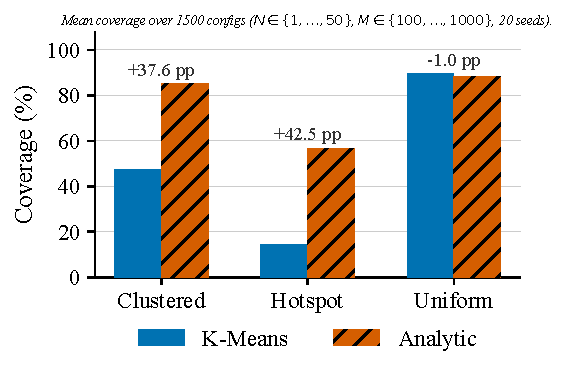
\includegraphics[width=\columnwidth, trim={0 3mm 0 7mm}, clip]{figures/fig_coverage_by_dist.pdf}
\caption{Mean coverage by user distribution across 1{,}500 synthetic configurations
($N\in\{1,\ldots,50\}$, $M\in\{100,\ldots,1000\}$, 20 seeds).
$\Delta$ annotations show Analytic\,$-$\,K-Means in percentage points.
Analytic wins 483/500 clustered and 485/500 hotspot configurations;
K-Means wins 320/500 uniform configurations.}
\label{fig:coverage_by_dist}
\end{figure}

On clustered and hotspot distributions the analytic heuristic gains $+37.6$ and $+42.5$ percentage points respectively, while simultaneously reducing interference.
On the uniform distribution, where users have no spatial structure, K-means with its fixed 150\,m altitude slightly outperforms the analytic heuristic ($89.5\%$ vs.\ $88.5\%$), because the altitude-adaptation formula infers large cluster spread and raises altitude, slightly widening beams. However, even on uniform distributions, the analytic heuristic overtakes K-means at $N \geq 41$ as interference accumulates ($+3.5$\,pp at $N{=}50$).
Overall, the analytic heuristic leads by $+26.3$\,pp across all 1{,}500 configurations. All build times are under 10\,ms.

\paragraph{Per-Configuration Breakdown.}
Fig.~\ref{fig:hotspot_vs_N} reveals the key asymmetry between methods as fleet size grows.
On the hotspot distribution, K-means coverage collapses rapidly, from $64.8\%$ at $N{=}5$ to effectively $0\%$ by $N{=}40$, because its fixed
150\,m altitude spreads beams too wide once drones become dense relative to the hotspot footprint,
leaving large fractions of users in inter-beam nulls.
The analytic heuristic adapts altitude to the inferred cluster spread, keeping beams focused and
sustaining $92.0\%$ at $N{=}5$ and still $22.1\%$ at $N{=}50$.
On clustered distributions, the analytic heuristic plateaus at approximately $80$--$83\%$ for $N \geq 10$, while K-means degrades monotonically from $94.2\%$ at $N{=}5$ to $12.0\%$ at $N{=}50$.

\begin{figure}[t]
\centering
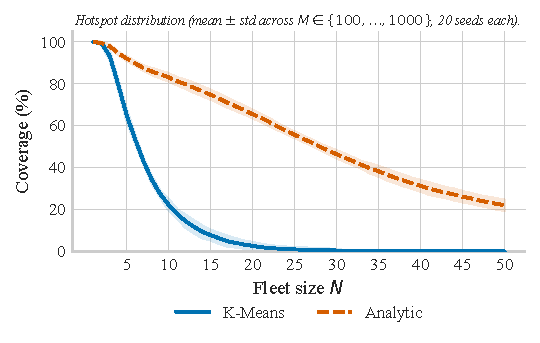
\includegraphics[width=\columnwidth, trim={0 3mm 0 5mm}, clip]{figures/fig_hotspot_vs_N.pdf}
\caption{Mean coverage vs.\ fleet size on the hotspot distribution, averaged over
$M\in\{100,\ldots,1000\}$ users and 20 seeds (shaded band: $\pm$1\,std across $M$).
K-Means coverage collapses as $N$ grows because the fixed 150\,m altitude spreads beams
too wide for the increasing drone density. The Analytic heuristic adapts altitude to cluster
geometry and sustains substantially higher coverage across the full $N{=}1$--$50$ range.}
\label{fig:hotspot_vs_N}
\end{figure}

\paragraph{Optimal Fleet Size.}
The extended sweep to $N{=}50$ reveals a striking divergence. On clustered distributions, the analytic heuristic plateaus near $80$--$83\%$ coverage for $N \geq 10$, losing only $15$\,pp from its $N{=}5$ value of $95.3\%$ even at $N{=}50$. K-means, by contrast, degrades monotonically from $94.2\%$ at $N{=}5$ to $12.0\%$ at $N{=}50$, a $68.2$\,pp gap. On hotspot distributions, K-means reaches $0\%$ coverage by $N{=}40$, while the analytic heuristic still covers $22.1\%$ of users at $N{=}50$. Even on uniform distributions, where K-means holds a mid-range advantage ($N \in [9, 40]$), the analytic heuristic overtakes K-means at $N{=}41$ as interference accumulates.

This confirms that altitude adaptation provides a robust defence against interference scaling: where K-means coverage collapses under co-channel interference at large fleet sizes, the analytic heuristic degrades gracefully.

%----------------------------------------------------------------------
\subsection{UL Orientation Validation}
\label{sec:orientation_validation}
%----------------------------------------------------------------------

\subsubsection{Experimental Setup}

To verify that the analytic nadir-pointing UL orientation is near-optimal, we conduct a per-drone angle sweep across all 36 configurations ($N \in \{5,10,15,20,25,30\}$, $M \in \{200, 400\}$, three distributions). Each drone's UL tilt and azimuth is optimized independently while all other drones are held at their method defaults, sweeping tilts $0^\circ$--$60^\circ$ (every $1^\circ$) and azimuths $0^\circ$--$355^\circ$ (every $5^\circ$), yielding 4{,}392 combinations per drone.

\subsubsection{Results}

The per-drone sweep optimises each drone's UL tilt and azimuth independently while all other drones are held at their defaults.
Table~\ref{tab:orientation_sweep} summarises the mean per-drone coverage gain (the improvement achievable by individually re-orienting any single drone) averaged over 36 configurations.

\begin{table}[t]
\centering
\caption{Mean Per-Drone Coverage Gain from Angle Optimisation (36 configurations, $N \in \{5\text{--}30\}$, $M \in \{200, 400\}$)}
\label{tab:orientation_sweep}
\begin{tabular}{@{}lccc@{}}
\toprule
Method & Mean $\Delta$Cov (pp) & Max $\Delta$Cov (pp) & Distribution \\
\midrule
Analytic (nadir) & $0.40$ & $0.78$ & uniform, $N{=}5$ \\
K-means (nadir)  & $0.77$ & $4.47$ & hotspot, $N{=}5$ \\
\bottomrule
\end{tabular}
\end{table}

The analytic nadir-pointing orientation leaves on average only $0.40$ percentage points of coverage to per-drone optimisation, with no single configuration exceeding $0.78$\,pp.
By contrast, the K-means nadir baseline leaves larger room for improvement, especially on hotspot distributions (up to $4.47$\,pp), because K-means centroids may not align with the densest user subregions after cluster splitting at large fleet sizes.
This confirms that for the analytic heuristic, where each drone is placed directly above its cluster centroid, nadir-pointing is near-optimal across all tested fleet sizes and distributions, leaving little room for per-drone fine-tuning.

%----------------------------------------------------------------------
\subsection{Real-World Validation}
\label{sec:results_telecom}
%----------------------------------------------------------------------

\subsubsection{Experimental Setup}

To validate the heuristics on realistic user distributions we use the Telecom Italia
Trentino dataset~\cite{barlacchi2015}, which records SMS, call,  and internet activity
in 10-minute bins for each $235 \times 235$\,m grid cell across the Trentino
province. For each (date, hour) pair we:
\begin{enumerate}[label=(\alph*)]
    \item Identify the $10 \times 10$-cell crop with the highest aggregate activity
          via a sliding-window maximum (hottest $2{,}350 \times 2{,}350$\,m patch).
    \item Sample 800 user positions from the crop, weighted by per-cell activity,
          and rescale to a $2{,}000 \times 2{,}000$\,m area.
\end{enumerate}

\textbf{Balanced snapshot design.}
We use a balanced $4 \times 2 \times 3$ factorial design over 24 snapshots:
\begin{itemize}
    \item \textbf{4 weeks:} early November (Nov~3--4), mid-November (Nov~9, 14), late November (Nov~20, 24), and mid-December (Dec~5, 8).
    \item \textbf{2 day types:} one weekday and one weekend day per week.
    \item \textbf{3 hours:} 10:00, 15:00, and 20:00 UTC, spanning morning, afternoon, and evening demand.
\end{itemize}
This design is balanced across temporal covariates (day-of-week, time-of-day, month) and spans a wide range of real-world spatial demand patterns.

\textbf{Replication and seed design.}
We use $R = 20$ seeds per condition. Each seed provides an independent K-means initialisation and independently subsamples $M$ users from the full 800-user pool for that snapshot, so seed variation captures both initialisation noise and sampling variation. All methods within a seed receive the \emph{same} user subsample, constituting a paired (within-block) design. This yields $24 \times 30 \times 8 \times 2 \times 20 = 230{,}400$ evaluations across 24 snapshots, $N \in \{1,\ldots,30\}$ drone counts, $M \in \{100,200,\ldots,800\}$ user levels, and 2 methods.

\subsubsection{Results}

Fig.~\ref{fig:telecom_coverage} presents mean coverage across
24 temporal snapshots from the Telecom Italia dataset, evaluated over 20 seeds at
$M = 800$ users per snapshot.

\begin{figure}[t]
\centering
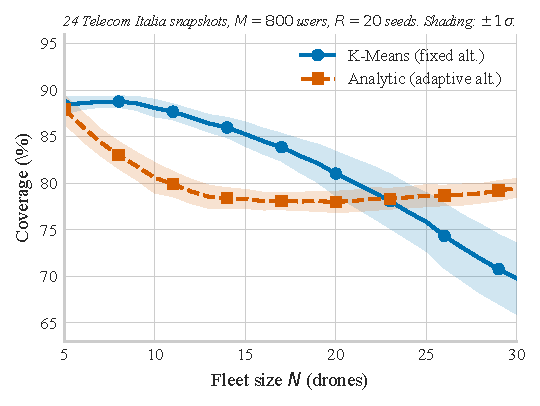
\includegraphics[width=\columnwidth, trim={0 3mm 0 5mm}, clip]{figures/fig_telecom_coverage_vs_N.pdf}
\caption{Coverage vs.\ fleet size $N$ averaged over 24 Telecom Italia snapshots
($M=800$ users, $R=20$ seeds). Shading denotes $\pm 1\,\sigma$ across snapshots.}
\label{fig:telecom_coverage}
\end{figure}

Several patterns emerge at $M{=}800$, where 5 drones must each serve on average 160 users:

\begin{itemize}
    \item \textbf{Coverage is non-monotone for K-means.} Coverage rises from 88.4\% at $N{=}5$ to a peak of 88.8\% at $N{=}8$, direct evidence that more drones do improve coverage when user load is high enough to benefit from additional spatial subdivision. Beyond $N{=}8$, coverage degrades monotonically to 69.7\% at $N{=}30$ ($-19.1$\,pp from the peak), driven by two compounding mechanisms: (i)~\emph{hotspot crowding}, where K-means splits existing clusters into sub-clusters rather than extending reach into sparser regions, concentrating more drones in a shrinking footprint; and (ii)~\emph{SINR collapse}, where drone proximity raises the co-channel interference floor, pulling previously-covered users below the $\gamma_r = 3\,\dB$ threshold. The fixed 150\,m altitude amplifies both effects by providing no vertical separation between interfering beams.
    \item \textbf{Analytic maintains a stable floor.} Coverage falls from 87.9\% at $N{=}5$ to a plateau of approximately 78\% for $N \in [12, 25]$, then partially recovers to 79.5\% at $N{=}30$. The adaptive per-drone altitude shrinks as clusters become denser with added drones, providing vertical beam separation that suppresses mutual interference and limits total coverage loss to only $-8.4$\,pp compared to $-19.1$\,pp for K-means.
    \item \textbf{Analytic surpasses K-means at $N \geq 23$.} The crossover occurs at $N{=}23$ (+0.3\,pp) and the advantage grows to $+9.7$\,pp at $N{=}30$, where interference management is most critical. This confirms that altitude adaptation, not horizontal placement, is the decisive differentiator at high drone densities.
\end{itemize}

%----------------------------------------------------------------------
\subsection{Discussion}
\label{sec:discussion}
%----------------------------------------------------------------------

The core reason K-means degrades at large fleet sizes is that its objective, minimizing within-cluster geometric distortion, is blind to the interference term in the SINR denominator. Adding drones near a demand hotspot tightens spatial coverage but simultaneously raises the interference floor for all nearby users, potentially pulling them below the coverage threshold even though their serving drone is closer. The analytic heuristic breaks this tradeoff through per-drone altitude adaptation: as clusters tighten, drones descend to narrow their beams and increase vertical separation from neighbours, suppressing co-channel interference without sacrificing proximity. This mechanism explains the widening advantage observed across both synthetic and real-world experiments as fleet size grows, and the non-monotone coverage curves imply a practical fleet-sizing constraint: beyond a density-dependent optimal~$N^*$, adding co-channel drones is counterproductive without frequency planning.

The heuristic inherits K-means horizontal placement and therefore shares its limitations on spatially uniform distributions, where the altitude formula infers large cluster spread and raises drones higher than necessary; this disadvantage reverses at large fleet sizes where interference suppression dominates. The MST backhaul topology minimizes total link distance rather than interference or throughput. Finally, the Telecom Italia evaluation covers 24~temporal snapshots at a single user density ($M{=}800$); broader validation across propagation environments and density levels would strengthen generalisation claims.

%----------------------------------------------------------------------
\section{Conclusion}
\label{sec:conclusion}
%----------------------------------------------------------------------

We presented a closed-form geometry-aware heuristic for UAV base station deployment that derives altitudes and antenna orientations directly from the antenna beamwidths and user geometry, at effectively zero computational cost.
Across 1{,}500 synthetic configurations and 24 real-world Telecom Italia snapshots, the heuristic consistently outperforms a K-means baseline, with the advantage growing as fleet size increases and co-channel interference accumulates.
The key mechanism is per-drone altitude adaptation, which provides vertical beam separation that suppresses mutual interference, sustaining coverage where the fixed-altitude baseline collapses.

Our results also reveal a coverage--interference boundary inherent to co-channel operation: beyond an optimal fleet size $N^*$, interference outweighs the benefit of spatial subdivision.
This boundary shifts with user density and highlights that frequency planning is essential for dense UAV deployments at scale.
Future work includes integrating frequency reuse into the analytic framework, extending to non-stationary user distributions with online replanning, and validation with measured antenna patterns.
The simulation code is publicly available online.\footnote{\texttt{https://github.com/jalmanea/geometrybaseduavcommpaper}}

%----------------------------------------------------------------------
\bibliographystyle{IEEEtran}
\bibliography{references}

\end{document}
